\documentclass[12pt,twoside]{book}
\usepackage{../../thesis}
\graphicspath{ {../../images/} }

\begin{document}

\chapter{Introduction}
In this chapter, I will introduce the logistic map as an example of a chaotic system, without defining what it means for a system to be ``chaotic''.
Next, I will discuss the origin of chaos.
At last, I discuss what ``chaos'' is.

\section{Our First Chaotic Map}

This is the equation for logistic map:
\begin{equation}
  L_{\mu}(x) = \mu x(1-x),
  \label{logistic}
\end{equation}
and the ``equivalent'' differential equation:
\begin{equation}
  \frac{dx}{dt} = \mu x(1-x)
  \label{logisticdiffeq}
\end{equation}
(In general, we can go between continuous and discrete models
\begin{align*}
  \frac{dx(t)}{dt} = G(x(t)) &\quad\mbox{(Continuous)} \\
  x(t + 1) = F(x(t)) &\quad\mbox{(Discrete)}
\end{align*}
by using the following approximation of the differential equation by mapping
\begin{equation*}
  \frac{dx(t)}{dt} \approx \frac{x(t_0 + (n+1)\Delta t) - x(t_0 + n \Delta t)}{\Delta t},
\end{equation*}
which leads to an approximation of the mapping by the differential equation
\begin{equation*}
  F(x(n)) \approx x(n) + \Delta t \cdot G(x(n))
\end{equation*}
.)
The only difference between equations \pref{logisticdiffeq} and \pref{logistic}

The differential equation \pref{logisticdiffeq} can be easily solved by separation of variables.
\begin{align*}
  \frac{dx}{x(1-x)} &= \mu dt \\  
  \left( \frac{1}{x} + \frac{1}{1-x} \right) dx &= \mu dt
\end{align*}
Then, suppose that $x(0) = x_0$, and integrate from $t = 0$ to $T$
\begin{align*}
  \int_{x_0}^{x(T)} \frac{1}{x} + \frac{1}{1-x} dx &= \int_0^T \mu dt \\
  \log{\frac{x(T)}{1-x(T)}} - \log{\frac{x_0}{1-x_0}} &= \mu T \\
  \frac{x(T)}{1-x(T)} &= \frac{x_0 e^{\mu T}}{1-x_0} \\
  (1-x_0)x(T) &= x_0 e^{\mu T} (1-x(T)) \\
  (1-x_0 + x_0 e^{\mu T})x(T) &= x_0 e^{\mu T}
\end{align*}

Thus, we have (with a slight change of notation)
\begin{equation}
  x(t) = \frac{x_0 e^{\mu t}}{1 - x_0 + x_0 e^{\mu t}}
  \label{eq:logisticdiffeqsoln}
\end{equation}

Change in the growth rate $\mu$ does not alter the bahaviour.
\begin{figure}[ht]
  \begin{center}
    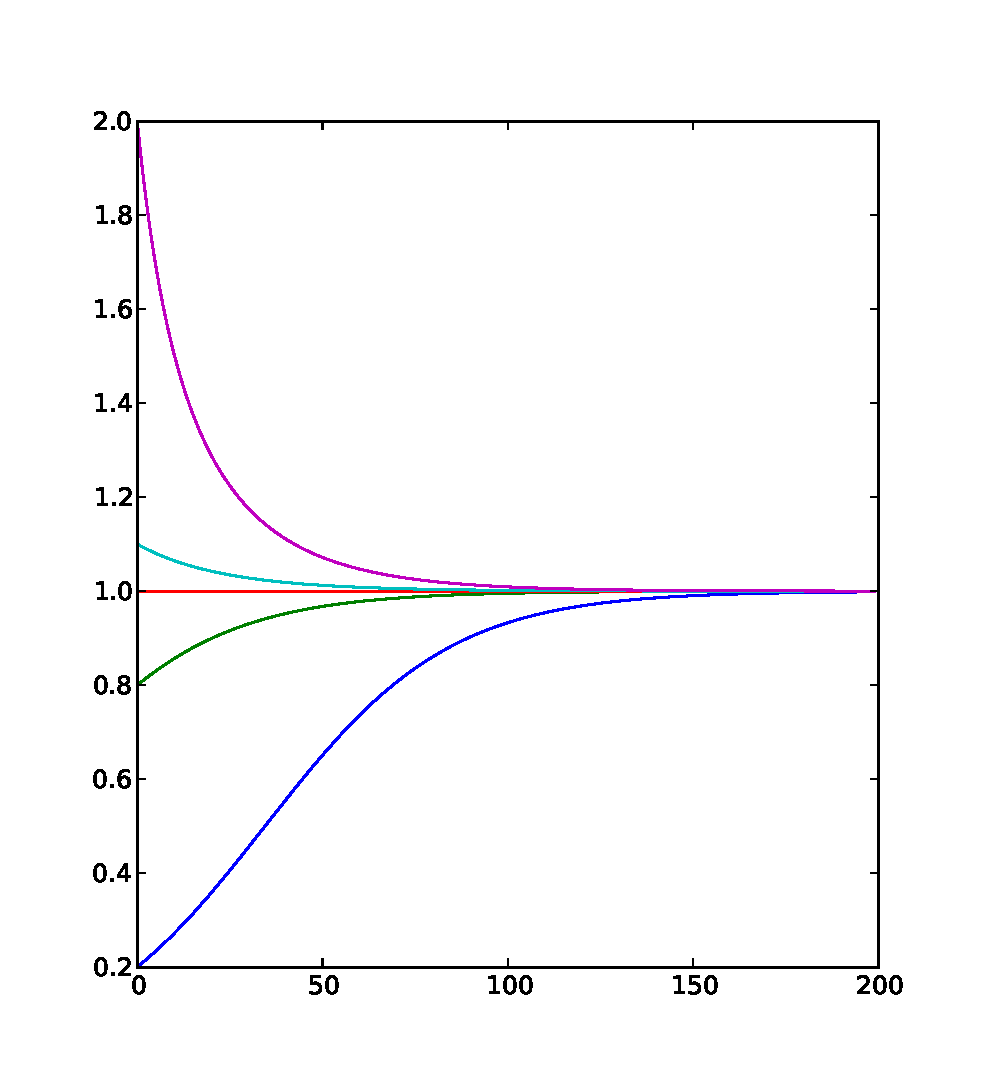
\includegraphics[scale=0.5]{logistic_diffeq_mu4_varyingx0}
  \end{center}
  \caption{
    Plot of equation \pref{eq:logisticdiffeqsoln} with $\mu = 4$ and various $x_0$. 
  Note that regardless of the initial value, $x(t)$ converges to $1$.
}
  \label{fig:logistic_diffeq1}
\end{figure}

%\begin{figure}[h]
%  \begin{center}
%    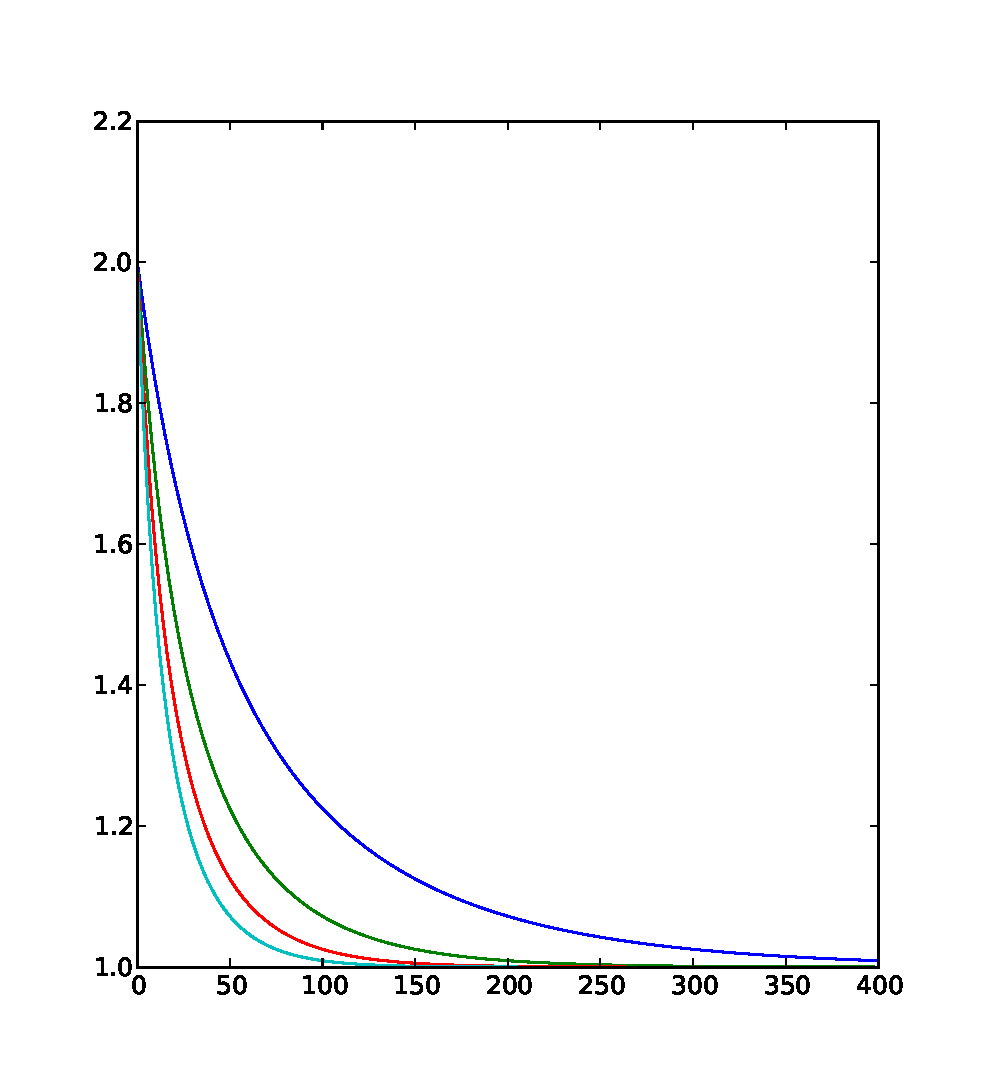
\includegraphics[scale=0.5]{logistic_diffeq_mu1234_x2}
%  \end{center}
%  \caption{
%    Plot of equation \pref{eq:logisticdiffeqsoln} with $x_0 = 2$ and various $\mu$ (1,2,3,4).
%    As $\mu$ increases, $x(t)$ converges to $1$ faster.
%    However, it does not alter the overall behaviour.
%  }
%  \label{fig:logistic_diffeq2}
%\end{figure}

\begin{figure}[h]
  \begin{center}
    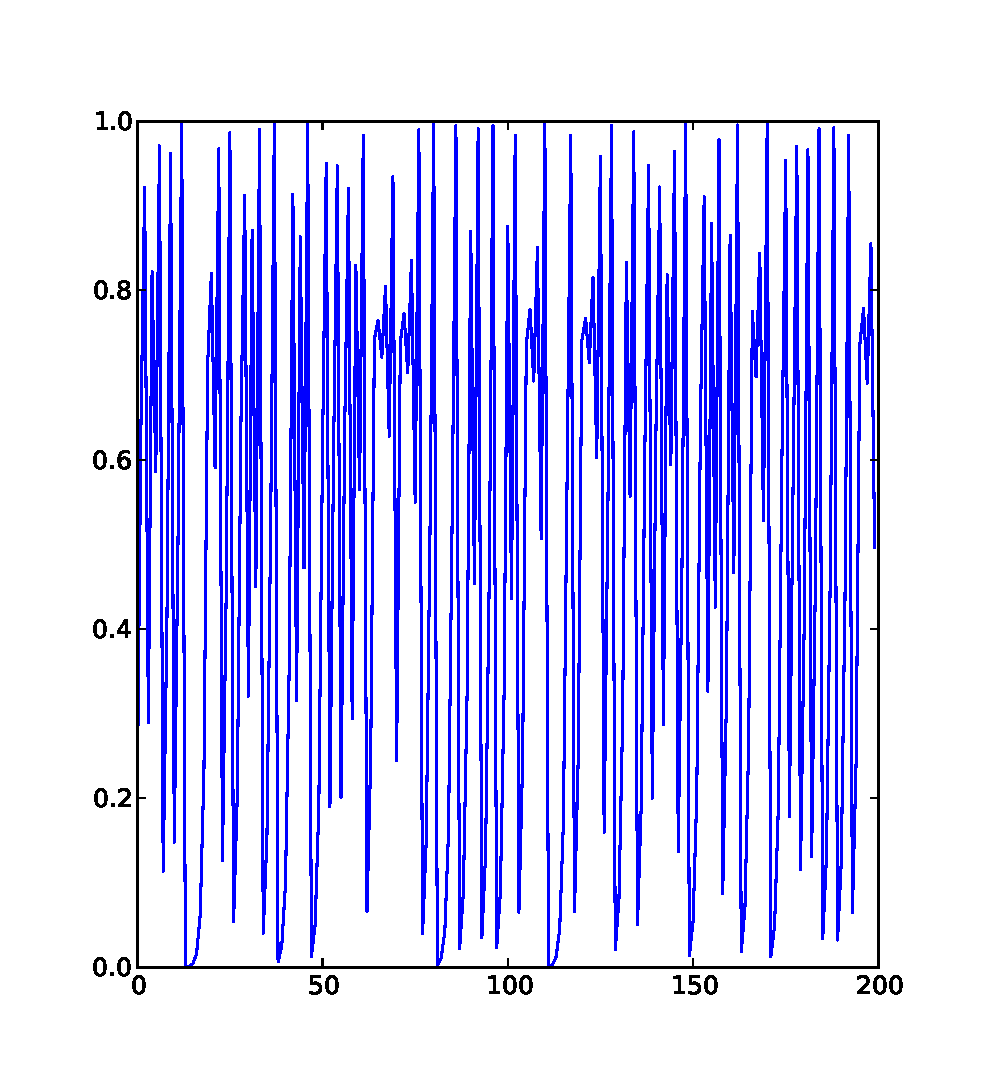
\includegraphics[scale=0.5]{logistic_map_mu4_x02}
  \end{center}
  \caption{
    Chaotic map.
  }
  \label{fig:logistic_map_chaotic}
\end{figure}


\section{The Origin of Chaos}
Edward Lorentz is often regarded as the first discoverer of chaos.
\begin{figure}[t]
  \begin{center}
    \includegraphics[scale=0.5]{golden_lorentz_attractor}
  \end{center}
  \caption{Lorentz Attractor}
  \label{fig:lorentz}
\end{figure}
He found chaotic behaviours through atmospheric simulations using twelve differential equations.
In his seminal article ``Deterministic Nonperiodic Flow'', Lorentz discusses the chaotic behavior of a system of three differential equations, which were reduced from the original twelve equations.
Yoshisuke Ueda, though lesser known, was also one of the first scientists to recognize chaotic behaviors
In 1961 (a sketch of the ``Japanese Attractor''), while Lorentz's paper was published in 1963.
David Ruelle, a prominent French chaos researcher, introduced Ueda in \citet{ruelle}.
\footnote{Doubtful of Ueda's result, Ueda's mentor did not allow publication of Ueda's result until 1970, seven years after the publication of ``Deterministic Nonperiodic Flow.''
Because of the strict hierarchical structure of the Japanese academia, the first author of Ueda's paper, ``On the Behavior of Self-Oscillatory Systems with External Force'', is his mentor.%\cite[p89]{sprott}
``He was the emperor of his laboratory, and yet outwardly he was a mild-mannered gentleman.
I believed at that time that his was the most feudalistic of any laboratory in the world, and the wall of his authority was impenetrable during his reign, and I still believe it.
But because of that, we were not swept away by worldly concerns and could concentrate on our research, being faithful to our own ideas.''
``After my report, at any rate, Prof. Urabe admonished me personally.
'What you saw was simply the essence of quasi-periodic oscillations,' he said.
'You are too young to make conceptual observations.'
% 君が見たのは単に概周期振動にすぎない。概念的な所見を述べるのは、若い君のやることじゃない。
% Your result is no more than an almost periodic oscillation. Don't form a selfish concept of steady states. \citep[p.141]{gleick} : from 'Random Phenomena Resulting from Nonlinearity in the System Described by Duffing's Equation' (1985) in its postscript
The existence of random oscillations (chaos) was so obvious in my mind, that the negative comment did not crush me.
Even so, I was deeply disappointed that no one understood it no matter how hard I tried to explain.\citep[p47]{ueda-abraham}
Ueda left the following remark: ``Chaos, though common phenomena in the nature, has been dismissed because of the difficulty to grasp its full notion.''\citep[p533]{gleick}
Either way, vigorous research activities on chaos only started in the 70's.}
The reason that I would like to discuss this scientist instead of Lorentz is not because he is the first scientist to see chaos.
The name ``Japanese Attractor'' was given by David Ruelle.(Les assracteurs etranges; Strange Attractors, 1980)
% Ueda: 最初はアナログコンピュータが故障したのかと思った。しかしすぐに、いやそんなことはないと悟った (in Chaos Avant-Garde?)
``I thought vaccum tubes were broken or something---a common issues with computers of those days.'' \citep{lorentzbook} %私はすぐに真空管が弱ったか何かの、よくあるコンピュータトラブルを疑ったが、修理を頼む前に、どこで間違いが起ったかだけでも調べてみることにした
``As I look back, I feel that after those long exhausting vigils in front of the analog computer, staring atits output, chaos had become a totally natural, everyday phenomenon in my mind.
People call chaos a new phenomenon, but it has always been around.
There's nothing new about it---only people did not notice it.''\cite[p27]{ueda-abraham}
%「カオス現象は、われわれが、日常、目にしているありふれた実在の自然現象であるにもかかわらず、その概念把握の困難さのために、かっては見過ごされてきた」
The true value in Ueda's findings lies in its settings.
While Lorentz's discovery of chaos was through computer simulation of a hypothetical model, Ueda's was through an analog computer, a physical, real-world system.
``analog computeres solve coupled nonlinear equations by mimicking a physical system.
The error properties of a particular digital integration scheme need not ever be considered.
Indeed, within the range of accuracy limited by the tolerance of the components, the unsystematic errors caused by the thermal fluctuations and electronic noise in an analog simulation can actually be useful; this is the case, for example, in qualitative studies of chaotic dynamical systems.
% Crutchfiled, Farmer, Huberman 'Fluctuations and simple chaotic dynamics'
% Crutchfield, Packard 'Symbolic dynamics of one dimensional maps: Entropies, finite precision, and noise'
Specifically, these fluctuations obliterate the detailed fine structure found in the mathematical description of chaos and thus effectively mimic the coarse-grained behavior that is observed in actual physical experiments in, for example, convecting fluids or nonlinear electronic circuits.
''\cite[p.383]{campbell}
Chaos in the nature is seen elsewhere:
Libchaber confirmed chaos via bifurcation in an experiment involving Helium.
Logistic map is used to model population dynamics.
Lorentz system was created as a simplified model for atmosphere.
NH3 lazer is known to show chaotic behavior \citep{kantz-schreiber}.
B-Z reaction

\section{So What Is Chaos, After All?}
We tend to label a dynamical systems as ``chaotic'' on an intuitive ground.
If the orbit looks (judged by our visual sense organ complex), the system is called chaotic.
In 1986, the Royal Society held an international conference on chaos and defined ``chaos'' as ``Stochastic behavior occurring in a deterministic system.'' \cite{stewart}
Two Russian physicists famously said "A strange attractor seems strange only to a stranger."
(Boris Chirikov, Felix Izrailev)\cite{lorentzbook}

``As an academic term, I do not find the word 'chaos' very appropriate.
But what shall we call it then?
My proposal has been 'randomly transitional phenomena''; I will explain this below.
The characteristics of chaos in a physical system can be summarized as follows:
- Random phenomena that occur in deterministic systems.
- Random phenomena whose short-term behavior is predictable.
- Random phenomena whose long-term behavior is unpredictable.
- Although the phenomena are irregular and unpredictable, chaos does have a definite structure.
The original meaning of chaos, I feel, is a ``total disorder and ultimate unpredictability.''
But as scientific terminology, the word ``chaos'' seems to overemphasize the unpredictability alone.
\ldots
Even so I have to use the word ``chaos'' here \ldots
It is a concise expression which has already filtered into people's minds, and therefore I have decided it is rather pointless to resist it.
\citep[24]{ueda-abraham}

% Li and Yorke's essay in Chaos Avant-Garde: on how chaos developed over a decade since Poincare (202)
``He [Robert May] adoped our [Li and Yorke] use of 'chaos' as a mathematical term, and \textit{Period three implies chaos} therefore began to attract considerable worldwide attention by his strong advocacy in talks and papers.
\ldots
As use of the word 'chaos' spread, it became a word people loved to hate: they didn't have a better word but didn't like chaos.''
\citep[205]{ueda-abraham}

Although there is no universally accepted definition of chaos, most experts would concur that chaos is the {\it aperiodic, long-term behavior of a bounded, deterministic system that exhibits sensitive dependence on initial conditions} (Sprott, p104)

Our goal is to find the sufficient conditions that give rise to complex orbit structures.

\bibliographystyle{../../bibliography/pjgsm}
\bibliography{../../bibliography/thesis}
\end{document}
